\documentclass[12pt,compress]{beamer}
\usepackage{movie15}
\usepackage{amsmath}
\usepackage{url}
\usepackage{ucs}
\usepackage[utf8x]{inputenc}
\usepackage[ngerman]{babel}
\usepackage{bbm}
\usepackage{ulem}
\usepackage{multicol}
\usepackage{setspace}
\usepackage{color}
\usepackage{hyperref}

\usetheme{Boadilla}
\setbeamertemplate{footline}%{infolines theme}

\usecolortheme{lily}
\useinnertheme{circles}
\setbeamercovered{transparent}
\beamertemplatenavigationsymbolsempty

\definecolor{darkgreen}{rgb}{0,0.5,0}

\hypersetup{
    bookmarks=true,
    unicode=true,
    pdftoolbar=true,
    pdfmenubar=true,
    pdffitwindow=false,
    pdfstartview={FitH},
    pdftitle={Logistische Abbildung},
    pdfauthor={Michael Hartmann},
    pdfsubject={Vortrag über die logistische Abbildung},
    pdfcreator={vim},
    pdfproducer={pdflatex},
    pdfkeywords={chaos} {logitische Abbildung},
    pdfnewwindow=true,
    colorlinks=true,
    linkcolor=black,
    citecolor=green,
    filecolor=magenta,
    urlcolor=darkgreen
}



\title{Chaos I: Die Logistische Abbildung}
\institute{Kaffeeseminar}
\author{Michael Hartmann}
\date{30. November 2015}


%\titlegraphic{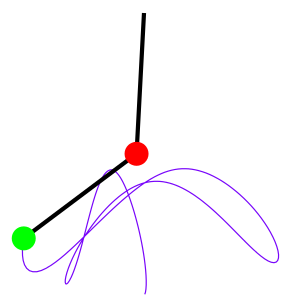
\includegraphics[scale=0.4]{title.png}}


\begin{document}

\begin{frame}
    \titlepage
\end{frame}

\frame {
    \frametitle{Abbildungen}

    Allgemeine Abbildung:
    \begin{equation}
    \nonumber
    X_{n+1} = F(X_n)
    \end{equation}

    \vfill

    Vorteile von Abbildungen:
    \begin{itemize}
    \item schnell für numerische Untersuchungen
    \item einfach für analytische Untersuchungen
    \item aus kontinuierlichen Systemen erhält man oft diskrete Abbildungen, z.B. Poincaré-Abbildungen
    \end{itemize}
}

\frame {
    \frametitle{Demographisches Modell}

    Modell für Enwicklung einer Population $X_n$:
    \begin{enumerate}
    \item Fortpflanzung:
    
    Population ist im Folgejahr um Faktor $q_f$ größer
    \item Verhungern:

    Population ist im Folgejahr um Faktor $(G-X_n)q_v$ geringer\\ ($G$: Maximalgröße)
    \end{enumerate}

    \begin{equation}
    \nonumber
    \Rightarrow X_{n+1} = q_f q_v X_n (G - X_n) \quad\quad\text{(logistische Gleichung)}
    \end{equation}
}

\frame {
    \frametitle{Logistische Gleichung}

    \begin{equation}
    \nonumber
    \Rightarrow X_{n+1} = q_f q_v X_n (G - X_n) \quad\quad\text{(logistische Gleichung)}
    \end{equation}

    \vfill

    Vereinfachungen:
    \begin{itemize}
    \item $x_n$ als Bruchteil der Maximalgröße $G$, $x_n = X_n/G$:
    \begin{equation}
    \nonumber
    \Rightarrow x_{n+1} = G q_f q_v (1 - x_n)
    \end{equation}

    \item Zusammenfassen der Parameter $\alpha \equiv G q_f qv$
    \begin{equation}
    \nonumber
    \Rightarrow x_{n+1} = \alpha (1 - x_n)
    \end{equation}
    \end{itemize}
}

\frame {
    \frametitle{Parameter $\alpha$}

    Logistische Abbildung:
    \begin{equation}
    \nonumber
    x_{n+1} = \alpha x_n(1-x_n)
    \end{equation}

    Extrema:
    \begin{align}
    \nonumber
    f^\prime(x_n) &= \alpha (1-2x_n) \quad \Leftrightarrow \quad x_n = \frac{1}{2} \quad \text{(Maximum)} \\
    \nonumber
    f\left(\frac{1}{2}\right) &= \frac{\alpha}{4} \quad \Leftrightarrow 0 \le \alpha \le 4
    \end{align}
}

\frame {
    \frametitle{Fixpunkte und Stabilität}

    Fixpunkte:
    \begin{equation}
    \nonumber
    f(x_s) = x_s \quad \Leftrightarrow \quad x_s = 0, \, x_s = 1-\frac{1}{\alpha}
    \end{equation}

    Stabilität:
    \begin{align}
    \nonumber
    x_{n+1} &= f(x_n) = f(x_s+\epsilon) \\
    \nonumber
            &\approx f(x_s) + \epsilon f^\prime(x_s) = x_s + \epsilon f^\prime(x_s)
    \end{align}

    $\Rightarrow$ Fixpunkt stabil für $|f^\prime(x_s)| < 1$
}

\frame {
    \frametitle{Stabilität von Fixpunkten}

    Ableitung der logistischen Gleichung:
    \begin{equation}
    \nonumber
    f^\prime(x_n) = \alpha (1-2x_n)
    \end{equation}

    Fixpunkt $x_s=0$:
    \begin{equation}
    \nonumber
    f^\prime(x_s=0) = \alpha \quad \Rightarrow \text{stabil für } \alpha < 1
    \end{equation}

    Fixpunkt $x_s=1-1/\alpha$:
    \begin{equation}
    \nonumber
    f^\prime(x_s=1-1/\alpha) = 2-\alpha \quad \Rightarrow \text{stabil für } 1 < \alpha < 3
    \end{equation}

    \hfill
    \only<2>
    {
    \begin{center}
    {\bf Was passiert für $\alpha>3$?}
    \end{center}
    }
}

\frame {
    \frametitle{Verhalten für $\alpha>3$}

    \begin{align}
    \nonumber
    f^2(x_n) &\equiv f(f(x_n)) \\
    \nonumber
    &= \alpha^2 \left( -\alpha x_n^4 + 2\alpha x_n^3 - (1+\alpha)x_n^2+x_n \right)
    \end{align}

    \begin{align}
    \nonumber
    f^2(x_s) = x_s \quad\Leftrightarrow \quad &x_s=0, \, x_s=1-1/\alpha, \\
    \nonumber
    &x_s = \frac{1}{2\alpha}\left(\alpha+1\pm\sqrt{\alpha^2-2\alpha-3}\right)
    \end{align}

    \begin{equation}
    \nonumber
    {f^2}^\prime(x_n) = \alpha^2 \left( -4\alpha x^3 + 6\alpha x^2 - 2 (1+\alpha)x_n +1 \right)
    \end{equation}

    \begin{equation}
    \nonumber
    {f^2}^\prime(x_s) = -\alpha^2+2\alpha+4 \quad\Rightarrow \alpha \le 1+\sqrt{6}
    \end{equation}
}

\frame {
    \frametitle{Spinnwebdiagramm}

    \begin{center}
    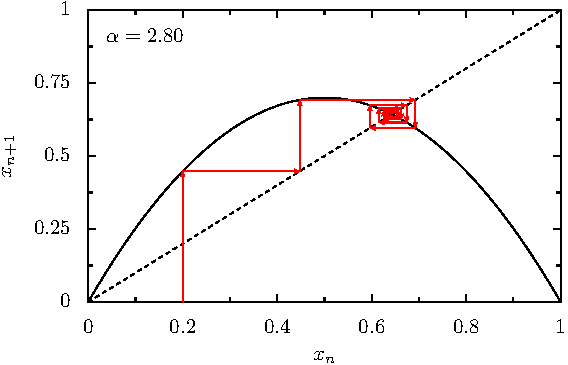
\includegraphics[scale=1.2]{coweb.pdf}
    \end{center}
}


\frame {
    \frametitle{Spinnwebdiagramm}

    \begin{center}
    \includemovie[poster,autoplay,controls=true]{8cm}{5.1875cm}{coweb.mp4}
    \end{center}
}

\frame {
    \frametitle{Plots}

    \begin{center}
    \only<1> { 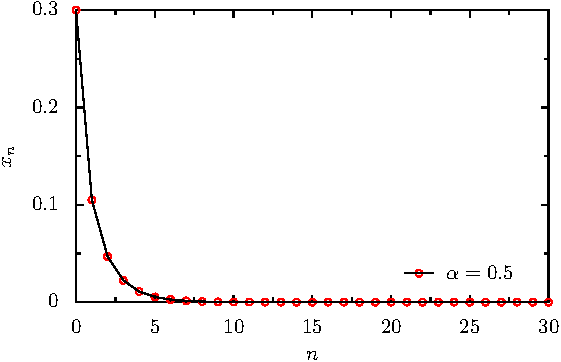
\includegraphics[scale=1.2]{plot1.pdf} }
    \only<2> { 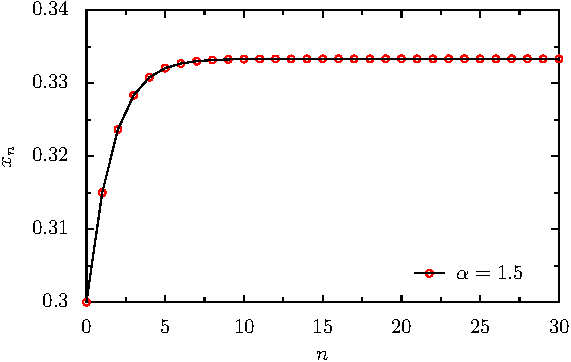
\includegraphics[scale=1.2]{plot2.pdf} }
    \only<3> { 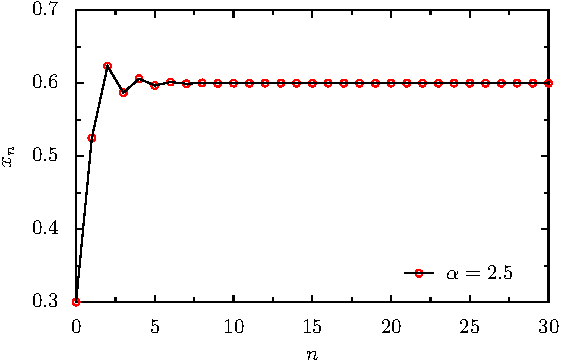
\includegraphics[scale=1.2]{plot3.pdf} }
    \only<4> { 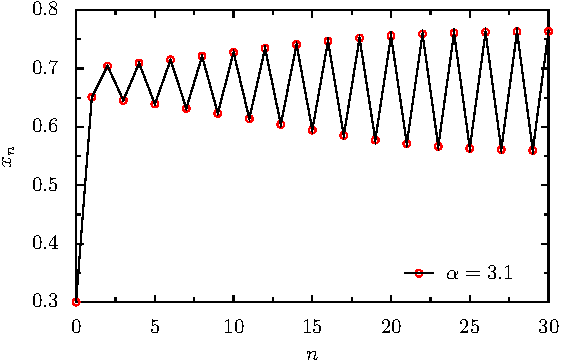
\includegraphics[scale=1.2]{plot4.pdf} }
    \only<5> { 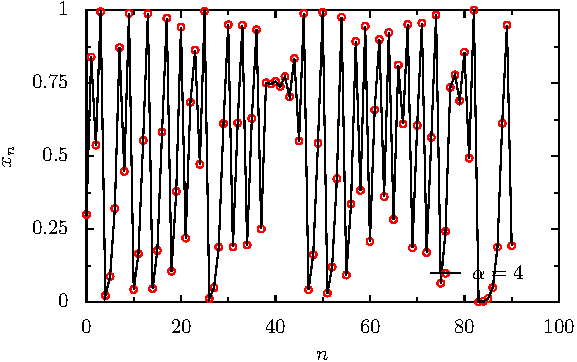
\includegraphics[scale=1.2]{plot5.pdf} }
    \end{center}
}

\frame {
    \frametitle{Bifurkationsdiagramm}

    \begin{block}{Bifurkationsdiagramm (Feigenbaumdiagramm)}
    Häufungspunkte des Systems in Abhängigkeit eines Parameters
    \end{block}

    \vfill
    \pause

    Algorithmus für logistische Abbildung:
    \begin{enumerate}
    \item Wähle Wert für Parameter $\alpha$, wähle einen Startwert $x_0$.
    \item Wende die logistische Abbildung $N$-mal an (z.B. $N=1000$).
    \item Berechne die Punkte $x_N, \dots, x_{N+n}$.
    \item Trage die berechneten Punkte ins Diagramm ein und wiederhole den Algorithmus für einen anderen Wert des Parameters $\alpha$.
    \end{enumerate}
}

\frame {
    \frametitle{Bifurkationsdiagramm}

    \begin{center}
    \only<1>
    {
    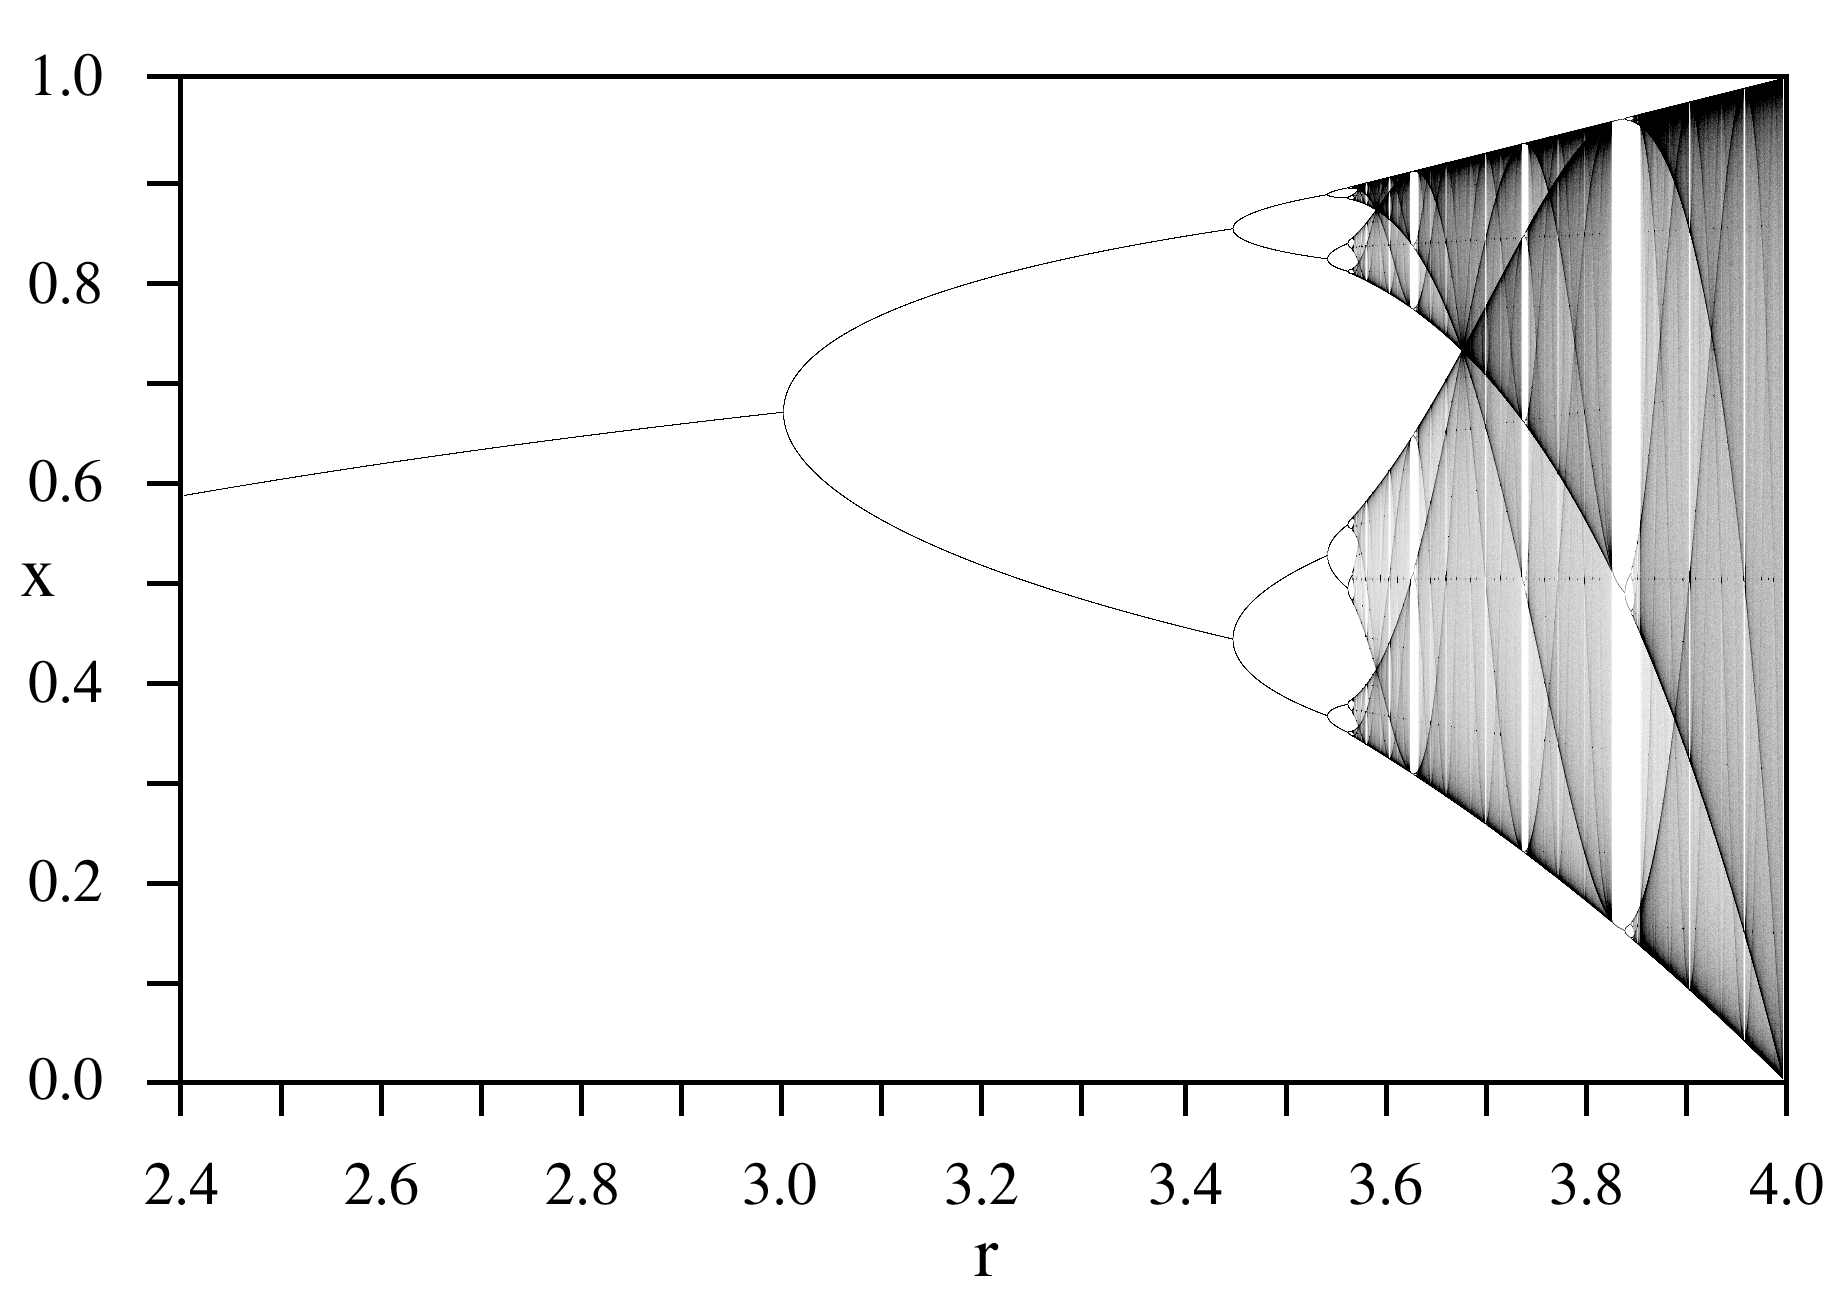
\includegraphics[scale=0.15]{bifurc1.png}
    }
    \only<2>
    {
    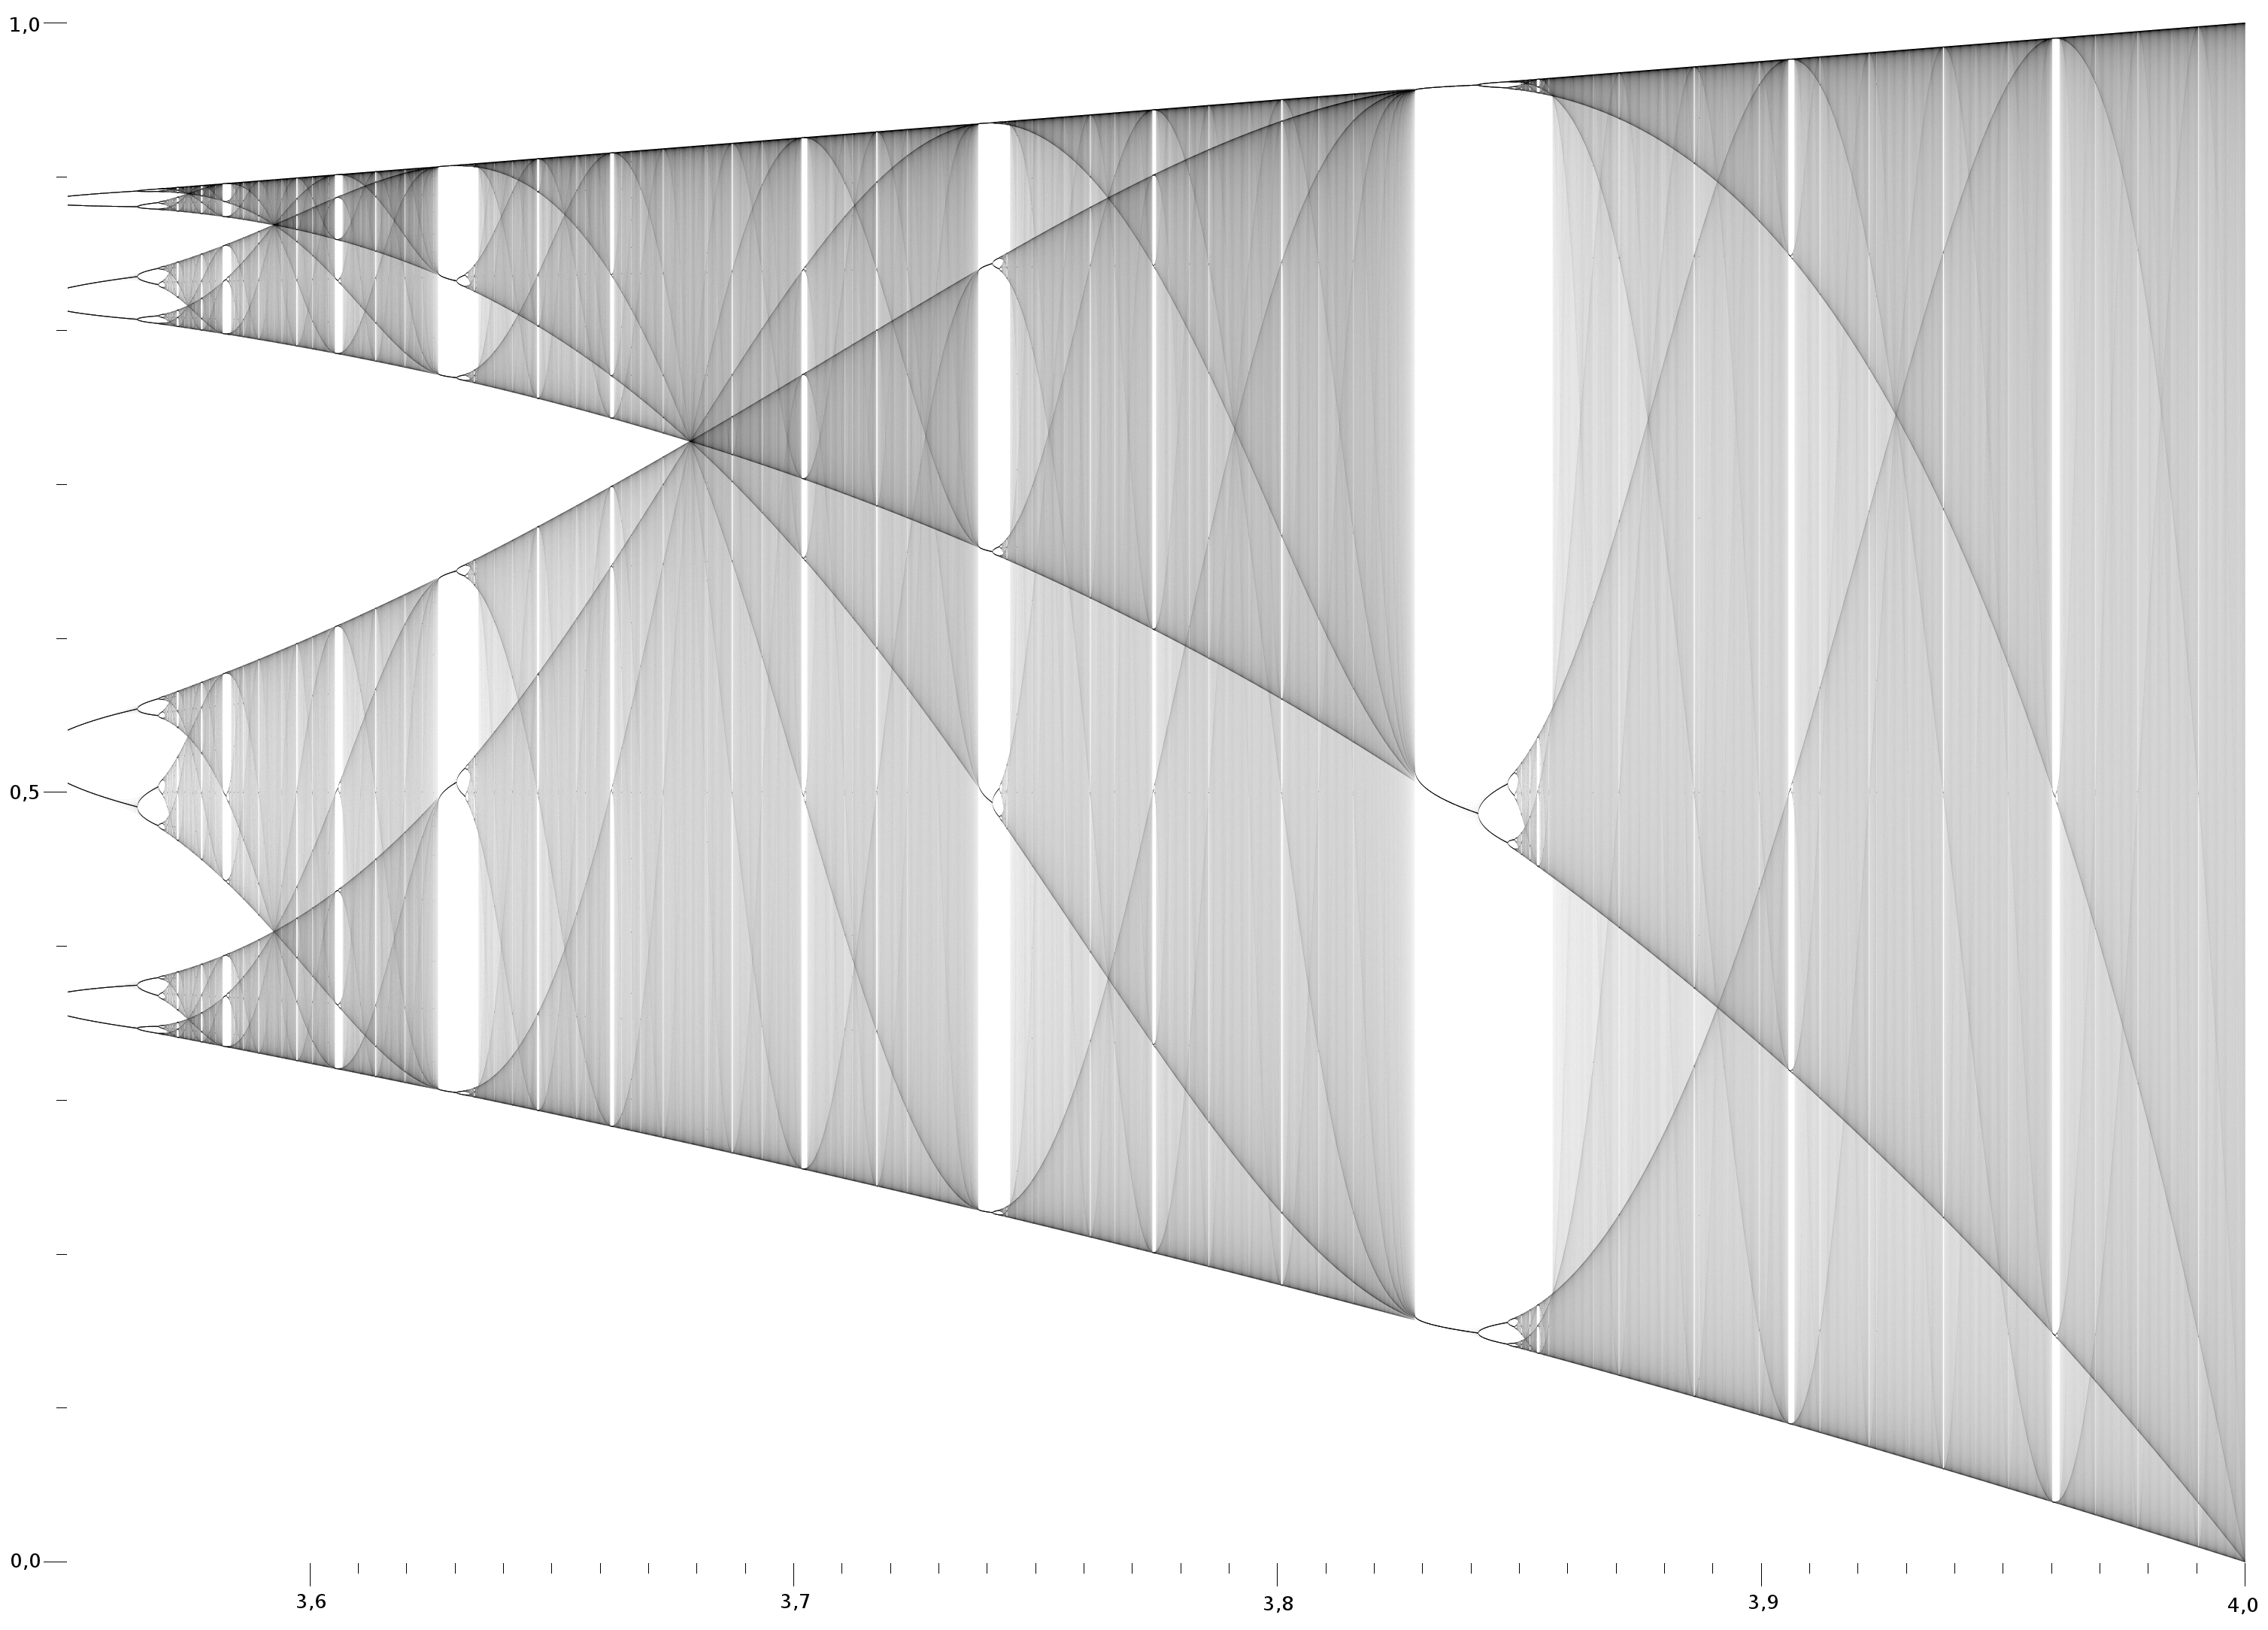
\includegraphics[scale=0.1]{bifurc2.png}
    }
    \end{center}

    \begin{flushright}
    {\small Bildquelle: \href{https://de.wikipedia.org/wiki/Logistische_Gleichung}{Wikipedia}}
    \end{flushright}
}

\frame {
    \frametitle{Invariante Dichte}

    Chaos bedeutet nicht Zufall! Z.B. $\alpha=4$:

    \vfill

    \begin{center}
    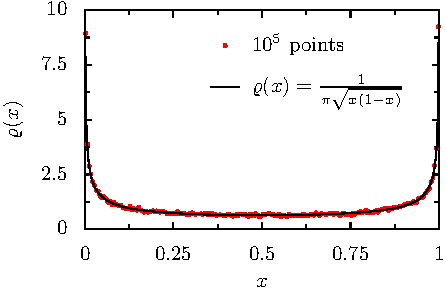
\includegraphics[scale=1.3]{invariantmeassure.pdf}
    \end{center}
}

\frame {

    \begin{center}
    \huge Vielen Dank für die Aufmerksamkeit!
    \end{center}
}


\end{document}
